\documentclass[11pt, reqno]{article}    % use "amsart" instead of "article" for AMSLaTeX format
\usepackage{my_packages}
\usepackage{tikz_packages}
\usepackage[american,siunitx]{circuitikz}
\usepackage{pgfplots}
\pgfplotsset{compat=1.14}
\usepackage[explicit]{titlesec}


\title{MAE 3145: PREDICT}
\author{Shankar Kulumani}
\date{Fall 2017}                          % Activate to display a given date or no date

\begin{document}
\begin{center}
{\Large \textbf{MAE3145: PREDICT}}
\end{center}
\subsection*{Description}
You are tasked to support teh elite Space Surveillance Reconstitution Team (SSRT) as an orbital analyst.
The SSRT will deploy to setup a remote space tracking capability when threat levels against the US indicate an attack in imminent.
As a SSRT member, it is your responsibility to develop software to locate satellite fom an Earth location.
In particular, SSRT's tacitcal terminal requires topocentric range, azimuth, and elevation to point its new secret tracking instruent.
Your program must compute and output this information at \underline{two minute intervals} each time the tactical \underline{terminal is in darkness} and the \underline{satellite is above the terminal's local horizon at a reasonable range}.
In addition, your program must determine if the statellite is visible to the tactical terminal, i.e. terminal in the dark, satellite illuminated by the sun, elevation angle greater than or equal to \SI{10}{\degree}, range less than \SI{1500}{\kilo\meter}.
If the satellite is in sunlight, SSRT members can operate teh terminal's new pointing instrument in one of three classified modes.

The SSRT's existence must be kept secret.
Thus, to validate your software \textbf{you must} view a low Earth orbiting satellite based on your program results.
In addition, if you know someone located at least \SI{100}{\kilo\meter} from our training site, and this person can be sworn to secrecy, give them your program results so they too can view a satellite.
Another person viewing a satellite based on yoru results will serve as a independent validation of your work.

As with all practical programming applications, there are three steps to this project:
\begin{enumerate}
    \item You will develop the correct algorithm and accomplish som hand calculations to provide a bsis to test your coded subroutines,
    \item You will code all subroutines, checking their output with that of your hand calculations to validate each subroutine as you go, eventually putting together the complete program and matching a provided single satellite data file perfectly,
    \item You will slightly alther this working program to accept a data file of hundres of real satellits, identify a viable vehicle to personally view, and go view it.
\end{enumerate}

The data required to run your program is located on \href{https://github.com/fdcl-gwu/MAE3145_library}{MAE3145: Astro Library}.
I will update these files throughout the semester.
The data comes from JSPOC's Two-Line Element Sets (TLEs), which are typically found in terms of three lines of data.
Each data set contains the 100+ brightest active payloads that JSPOC tracks.
However, not all satellites will be visible to the naked eye.

The TLE files are given in a very specifc format. 
The following describes each paramerter contained in the TLEs.
Some of these numbers will not be used in your program. 
You may also get teh latest TLEs yourself at \href{www.clestrak.com}{celestrak.com}.
There are many references for the TLE description available in textbooks or online, but one is available \href{https://goo.gl/W6MZb2}{https://goo.gl/W6MZb2}.

\begin{figure}
    \centering
    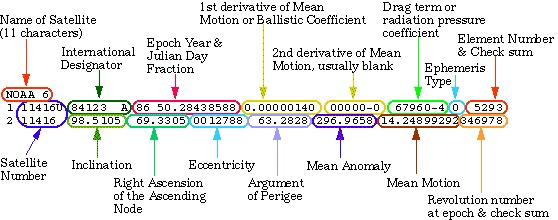
\includegraphics[width=\textwidth, keepaspectratio]{figures/tle.jpeg}
    \caption{TLE Format \label{fig:tle}}
\end{figure}
\end{document}  
